\documentclass[../../main.tex]{subfiles}

\begin{document}

\subsubsection*{Umfrage-Parameter}
\addcontentsline{toc}{subsubsection}{Umfrage-Parameter}

\begin{sloppypar}
Die Online-Umfrage wurde zwischen dem 4. und dem 18. Juli 2016 durchgeführt. Von insgesamt 994 eingeladenen Teilnehmer nahmen 324 an der Befragung teil. Die erreichte Rücklaufquote liegt bei 33\%
\end{sloppypar}

\subsubsection*{Auswertung Allgemeine Fragen}
\addcontentsline{toc}{subsubsection}{Auswertung Allgemeine Fragen}

\subparagraph*{Frage: Rolle im Unternehmen}\mbox{}
\begin{figure}[H]
\centering
\framebox[\textwidth]{\scriptsize $n: 323$}
\framebox[\textwidth]{\scalebox{0.9}{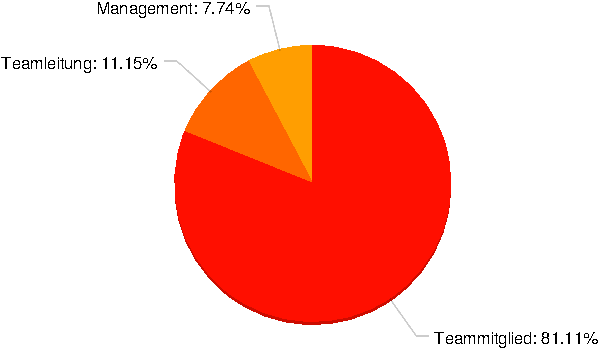
\includegraphics{figures/esurvey/c_allg_p1_rolle_im_unternehmen}}}
\caption{Auswertung Frage P1}
\label{P1}
\end{figure}

\subparagraph*{Frage: Bereichszugehörigkeit}\mbox{}
\begin{figure}[H]
\centering
\framebox[\textwidth]{\scriptsize $n: 323$}
\framebox[\textwidth]{\scalebox{0.9}{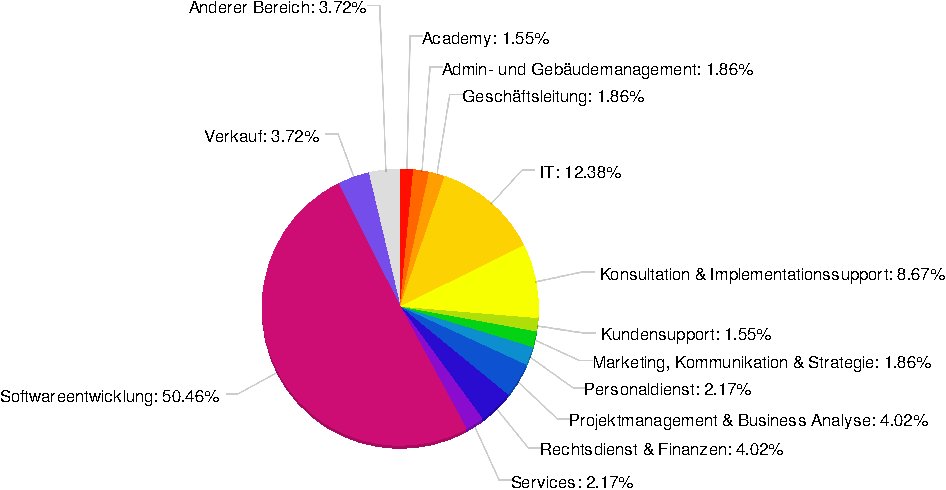
\includegraphics{figures/esurvey/c_allg_p2_bereiche}}}
\caption{Auswertung Frage P2}
\label{P2}
\end{figure}

\subparagraph*{Frage: Jahre beim Unternehmen}\mbox{}
\begin{figure}[H]
\centering
\framebox[\textwidth]{\scriptsize $n: 322$}
\framebox[\textwidth]{\scalebox{0.9}{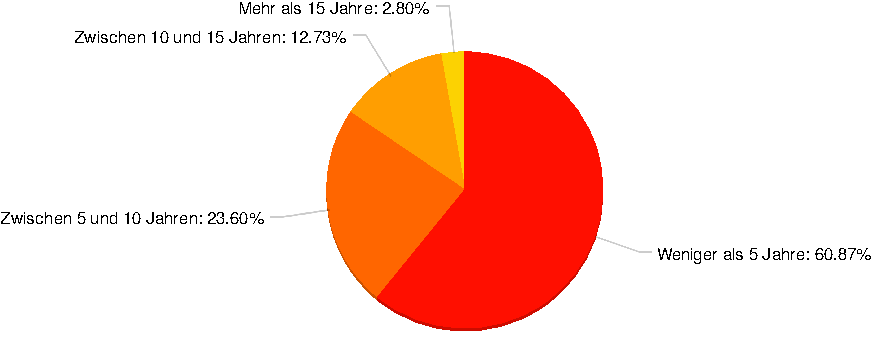
\includegraphics{figures/esurvey/c_allg_p3_firmenjahre}}}
\caption{Auswertung Frage P3}
\label{P3}
\end{figure}

\subparagraph*{Frage:Jahre in der Branche}\mbox{}
\begin{figure}[H]
\centering
\framebox[\textwidth]{\scriptsize $n: 322$}
\framebox[\textwidth]{\scalebox{0.9}{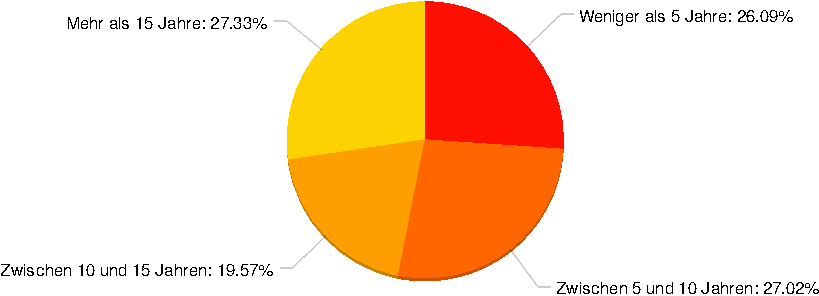
\includegraphics{figures/esurvey/c_allg_p4_branchenjahre}}}
\caption{Auswertung Frage P4}
\label{P4}
\end{figure}

\subparagraph*{Frage: Höchster Schulabschluss}\mbox{}
\begin{figure}[H]
\centering
\framebox[\textwidth]{\scriptsize $n: 322$}
\framebox[\textwidth]{\scalebox{0.9}{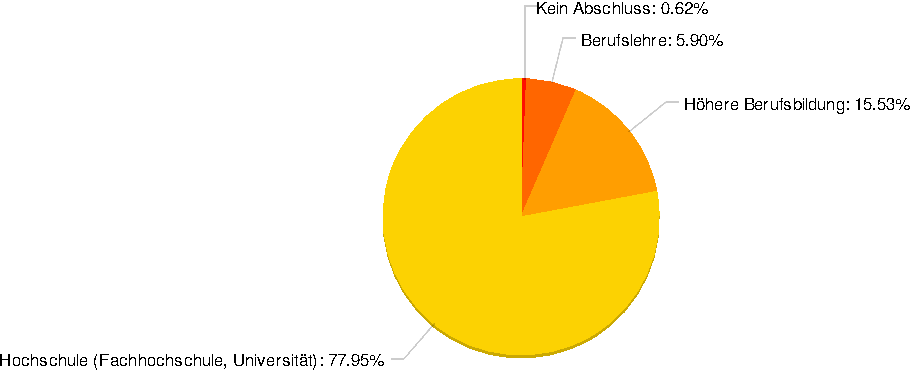
\includegraphics{figures/esurvey/c_allg_p5_schulabschluss}}}
\caption{Auswertung Frage P5}
\label{P5}
\end{figure}

\subparagraph*{Frage: Herkunft (Weltregion)}\mbox{}
\begin{figure}[H]
\centering
\framebox[\textwidth]{\scriptsize $n: 322$}
\framebox[\textwidth]{\scalebox{0.9}{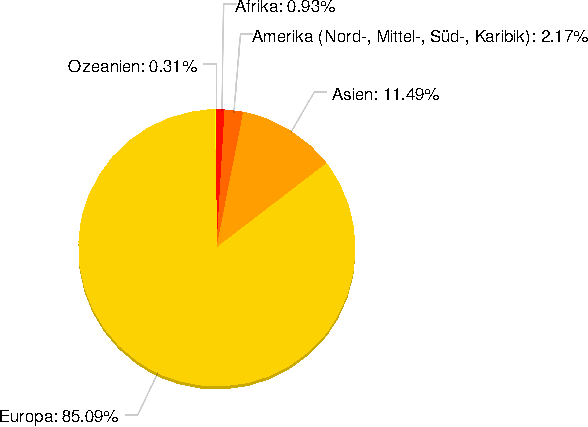
\includegraphics{figures/esurvey/c_allg_p6_weltregion}}}
\caption{Auswertung Frage P6}
\label{P6}
\end{figure}

\end{document}
